\documentclass[a4paper]{scrartcl}
\usepackage{scrpage2}
\usepackage[ngerman]{babel}
\usepackage[T1]{fontenc}
\usepackage[utf8]{inputenc}
%\usepackage[pdftex]{graphicx}
%\usepackage[intlimits]{amsmath}
%\usepackage{listings}
%\lstset{frame=single,breaklines=true}
\usepackage{ amssymb }
\usepackage{amsmath}
\usepackage{hyperref}
\usepackage{enumerate}
\usepackage[a4paper, total={19cm, 23cm}]{geometry}
\usepackage{stmaryrd}
\usepackage{esvect}
\usepackage{graphicx}
\pagestyle{scrheadings}
\pagenumbering{gobble}
\ihead{Übungsblatt 5\\Nils Werner 108012219293}
\chead{\\Paul Rösler 108012225686	}
\ohead{Übungsgruppe: Mo. 16:00\\Daniel Teuchert 108012214552}
\setheadsepline{0.4pt}
\begin{document}

\section*{Aufgabe 1}

\newpage
\section*{Aufgabe 2}
\begin{enumerate}[a)]
\item
$R_2, R_3:$\\
$R_2=F_{2\pi 2^{-2}}=F_{\frac{\pi}{2}} = 
\begin{pmatrix}
1 & 0 \\ 0 & e^{\frac{i \pi}{2}} \\
\end{pmatrix} = 
\begin{pmatrix}
1 & 0 \\ 0 & cos(\frac{\pi}{2})+i~sin(\frac{\pi}{2})\\
\end{pmatrix}$ \\
$R_3=F_{\frac{\pi}{4}} = 
\begin{pmatrix}
1 & 0 \\ 0 & e^{\frac{i \pi}{4}} \\
\end{pmatrix} = 
\begin{pmatrix}
1 & 0 \\ 0 & cos(\frac{\pi}{4})+i~sin(\frac{\pi}{4})\\
\end{pmatrix}$ \\
Eigentlich werden kontrollierte $R_k^{-1}$ für die QFT$_{2^n}^{-1}$ benötigt.

\item Für $|z\rangle = |z_1 z_2 z_3\rangle= (\frac{|0\rangle+e^{2\pi i0.x_3} |1\rangle }{\sqrt{2}})\bigotimes(\frac{|0\rangle+e^{2\pi i0.x_2x_3} |1\rangle }{\sqrt{2}})\bigotimes(\frac{|0\rangle+e^{2\pi i0.x_1x_2x_3} |1\rangle }{\sqrt{2}})$ gilt:

\begin{figure}[htp] \centering{
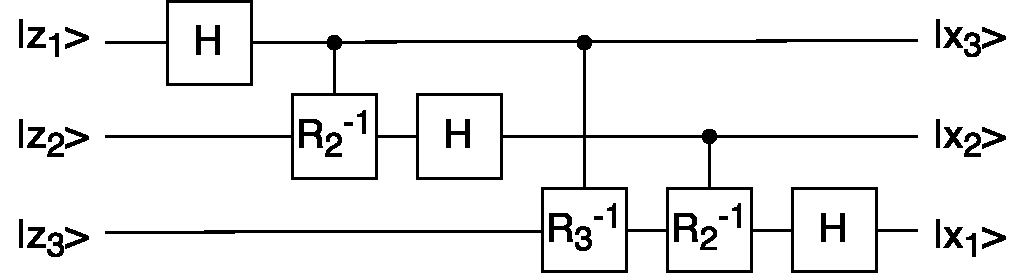
\includegraphics[scale=0.5]{A52b.pdf}}
\caption{Quantenschaltkreis für QFT$_{8}^{-1}$}
\end{figure}

\item Die Matrizen der folgenden unitären Abbildungen sind bekannt oder können wie folgt berechnet werden:\\
$H=\frac{1}{\sqrt{2}}\begin{pmatrix} 1 & 1\\ 1 & -1\\\end{pmatrix}$\\
$R_k^{-1}=(R_k^{*})^T=\begin{pmatrix} 1 & 0\\ 0 & cos(\frac{\pi}{2^{k-1}})-i~sin(\frac{\pi}{2^{k-1}})\\\end{pmatrix}$ da unitäre Abbildung.\\
Kontrolliertes $R_k^{-1}$ nach gleichem Schema wie $CNOT$:\\
$CR_2^{-1}=
\begin{pmatrix} 1 & 0 & 0 & 0\\
0 & 1 & 0 & 0\\
0 & 0 & 1 & 0\\
0 & 0 & 0 & \alpha_2\\\end{pmatrix}, CR_3^{-1}=
\begin{pmatrix}
1 & 0 & 0 & 0 & 0 & 0 & 0 & 0\\
0 & 1 & 0 & 0 & 0 & 0 & 0 & 0\\
0 & 0 & 1 & 0 & 0 & 0 & 0 & 0\\
0 & 0 & 0 & 1 & 0 & 0 & 0 & 0\\
0 & 0 & 0 & 0 & 1 & 0 & 0 & 0\\
0 & 0 & 0 & 0 & 0 & \alpha_3 & 0 & 0\\
0 & 0 & 0 & 0 & 0 & 0 & 1 & 0\\
0 & 0 & 0 & 0 & 0 & 0 & 0 & \alpha_3\\\end{pmatrix}, \alpha_k = cos(\frac{\pi}{2^{k-1}})-i~sin(\frac{\pi}{2^{k-1}})$\\

$QFT_8^{-1}=(H\bigotimes I_2)(CR_2^{-1}\bigotimes I_1)(I_1\bigotimes H \bigotimes I_1)CR_3^{-1}(I_1 \bigotimes CR_2^{-1})(I_2 \bigotimes H)$\\
$=((H\bigotimes I_1)CR_2^{-1}(I_1\bigotimes H)) \bigotimes I_1)CR_3^{-1}(I_1 \bigotimes (CR_2^{-1}(I_1 \bigotimes H))$\\
$=\frac{1}{\sqrt{2^3}}(\begin{pmatrix} 1&1&1&1\\ 1&-1&\alpha_2&-\alpha_2\\ 1&1&-1&-1\\ 1&-1&-\alpha_2&\alpha_2\\\end{pmatrix} \bigotimes I_1) CR_3^{-1}(I_1 \bigotimes \begin{pmatrix}1&1&0&0\\ 1&-1&0&0\\ 0&0&1&1\\ 0&0&\alpha_2&-\alpha_2\\ \end{pmatrix})$\\
$=\frac{1}{\sqrt{2^3}}\begin{pmatrix}
1&0&1&0&1&0&1&0\\
0&1&0&1&0&1&0&1\\
1&0&-1&0&\alpha_2&0&-\alpha_2&0\\
0&1&0&-1&0&\alpha_2&0&-\alpha_2\\
1&0&1&0&-1&0&-1&0\\
0&1&0&1&0&-1&0&-1\\
1&0&-1&0&-\alpha_2&0&\alpha_2&0\\
0&1&0&-1&0&-\alpha_2&0&\alpha_2\\
\end{pmatrix}
CR_3^{-1}
\begin{pmatrix}
1&1&0&0&0&0&0&0\\
1&-1&0&0&0&0&0&0\\
0&0&1&1&0&0&0&0\\
0&0&\alpha_2&-\alpha_2&0&0&0&0\\
0&0&0&0&1&1&0&0\\
0&0&0&0&1&-1&0&0\\
0&0&0&0&0&0&1&1\\
0&0&0&0&0&0&\alpha_2&-\alpha_2\\
\end{pmatrix}$\\

\end{enumerate}

\newpage
\section*{Aufgabe 3}
\begin{figure}[htp] \centering{
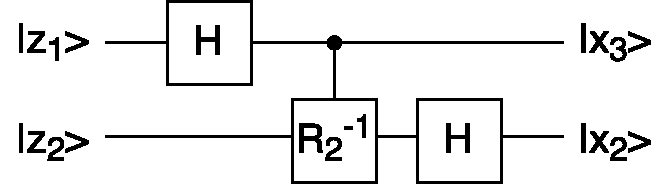
\includegraphics[scale=0.5]{A53.pdf}}
\caption{Quantenschaltkreis für QFT$_{4}^{-1}$}
\end{figure}

$|z\rangle = \frac{1}{2} (|0\rangle + |1\rangle - |2\rangle - |3\rangle) = \frac{1}{2} \begin{pmatrix} 1\\1\\-1\\-1\\\end{pmatrix} = \frac{1}{2} \begin{pmatrix} 1\\-1\\\end{pmatrix} \bigotimes \begin{pmatrix} 1\\1\\\end{pmatrix}$\\
$\xrightarrow{H\bigotimes I_1} \frac{1}{\sqrt{2}} \begin{pmatrix} 0\\1\\\end{pmatrix} \bigotimes \begin{pmatrix} 1\\1\\\end{pmatrix}$\\
$\xrightarrow{CR_2^{-1}}\frac{1}{\sqrt{2}} \begin{pmatrix} 0\\1\\\end{pmatrix} \bigotimes \begin{pmatrix} 1\\-i\\\end{pmatrix}$\\
$\xrightarrow{I_1\bigotimes H} \frac{1}{2} \begin{pmatrix} 0\\1\\\end{pmatrix} \bigotimes \begin{pmatrix} 1-i\\1+i\\\end{pmatrix} = \frac{1}{2}\begin{pmatrix} 0\\0\\1-i\\1+i\\\end{pmatrix} = \frac{1}{2} ((1-i)|2\rangle + (1+i)|3\rangle)$\\

\newpage
\section*{Aufgabe 4}

\end{document}
